\documentclass{beamer}
\usepackage{ctex, hyperref}
\usepackage[T1]{fontenc}

% other packages
\usepackage{latexsym,amsmath,xcolor,multicol,booktabs,calligra}
\usepackage{graphicx,pstricks,listings,stackengine}
\usepackage{caption, subfigure, multirow}

% xmu beamer (Keeping your original package reference)
\usepackage[blue]{TongjiBeamer}

\author[DeepMind]{小组:李致远、冯文喆、魏睿、宋泽顷、周启民}
\title{AlphaTensor}
\subtitle{Discovering faster matrix multiplication algorithms with reinforcement learning}
\institute{同济大学物理科学与工程学院}
\date{\today}

% defs
\def\cmd#1{\texttt{\color{red}\footnotesize $\backslash$#1}}
\def\env#1{\texttt{\color{blue}\footnotesize #1}}

\lstset{
    basicstyle=\ttfamily\small,
    keywordstyle=\bfseries\color{red!0!green!0!blue!100},
    emphstyle=\ttfamily\color{red!100!green!0!blue!0},
    stringstyle=\color{red!0!green!100!blue!0},
    numbers=left,
    numberstyle=\small\color{gray!50},
    rulesepcolor=\color{red!20!green!20!blue!20},
    frame=shadowbox
}

\begin{document}

\begin{frame}
    \titlepage
    \begin{figure}[htpb]
       \begin{center}
            \includegraphics[width=0.2\linewidth]{pic/tongji_logo.png}
        \end{center}
    \end{figure}
\end{frame}

\begin{frame}
    \tableofcontents[sectionstyle=show,subsectionstyle=show/shaded/hide,subsubsectionstyle=show/shaded/hide]
\end{frame}

% =======================================================
\section{背景介绍}

\begin{frame}{为什么选择这篇文章?}
    \begin{itemize}
        \item\textbf{本文作者},是 \textcolor{blue}{Google DeepMind} 团队的研究员。
        \begin{itemize}
            \item DeepMind 是人工智能领域的领军机构(AlphaGo、AlphaFold 等),DeepMind 团队联合创始人获得2024诺贝尔化学奖。
        \end{itemize}
        \item\textbf{学术影响力},论文发表在\textcolor{red}{\textbf{Nature(2022)}},引用次数超过 \textcolor{red}{\textbf{500}},github star超过 \textcolor{red}{\textbf{2800}}。
    \end{itemize}
    \vspace{0.3cm}
    \begin{center}
        \includegraphics[width=0.9\textwidth]{images/alphatensor_connected.png}
    \end{center}
\end{frame}

\begin{frame}{AlphaTensor 概述}
    \begin{block}{核心理念}
        “Discovering faster matrix multiplication algorithms with reinforcement learning”利用强化学习对矩阵乘法流程进行自动设计。
    \end{block}
    
    \vspace{0.5cm}
    
    \begin{itemize}
        \item \textbf{问题描述}:将一个矩阵乘法与一个张量 $T_n = \sum_{r=1}^{R} u^{(r)} \otimes v^{(r)} \otimes w^{(r)}$ 构建映射。
        \item \textbf{解法思路}:沿用alphazero强化学习的基本架构,通过多次自我博弈,找到矩阵 $T_n$ 的最小的低秩分解。
        \item \textbf{解法细节}:基于transformer架构。对矩阵 $T_n$ 提取嵌入特征后,用策略头与价值头计算下一步的秩-1分解与得分。使用MCTS剪枝搜索,产出一个完整的低秩分解。
    \end{itemize}
\end{frame}

\begin{frame}{为什么关注矩阵乘法?}
    \begin{itemize}
        \item \textbf{核心地位},矩阵乘法是深度学习(全连接层、Conv层、transformer层)和科学计算的基石。
        \item \textbf{优化维度}
        \begin{itemize}
            \item \emph{System角度}:向量化、访存优化(Cache命中)、并行计算。
            \item \emph{Math角度(本文研究方向)}:因为乘法开销 $\gg$ 加法开销,减少数值乘法的计算次数能显著提升性能。
        \end{itemize}
    \end{itemize}
    \begin{alertblock}{Strassen算法的启示 (1969)}
        对于 $2 \times 2$ 矩阵乘法:
        \begin{itemize}
            \item \textbf{朴素算法}:需要 \textbf{8次} 乘法 ($O(N^3)$)。
            \item \textbf{Strassen算法}:只需要 \textbf{7次} 乘法 ($O(N^{2.807})$)。
        \end{itemize}
        这意味着通过改变算法流程,可以在数学层面实现加速。
    \end{alertblock}
\end{frame}

\begin{frame}{Strassen算法的启示}
    \begin{columns}[T]
        \begin{column}{0.55\textwidth}
            \begin{itemize}
                \item \textbf{硬件层面的动机}:
                \begin{itemize}
                    \item 可以简单理解为,乘法器就是由加法器堆叠起来的。
                    \item 执行乘法的时间是加法的约 \textcolor{red}{\textbf{3.5倍}}。
                    \item 减少乘法次数 = 实际性能提升
                \end{itemize}
                
                \vspace{0.5cm}
                
                \item \textbf{Strassen的贡献 (1969)}:
                \begin{itemize}
                    \item 将 $2 \times 2$ 矩阵乘法从 \textbf{8次} 降至 \textbf{7次},大矩阵可以递归拆分为 $2 \times 2$ 子矩阵。
                    \item 复杂度:$O(N^3) \rightarrow O(N^{2.807})$
                \end{itemize}
            \end{itemize}
        \end{column}
        
        \begin{column}{0.60\textwidth}
            \vspace{-20pt}
            \begin{center}
                \includegraphics[width=\textwidth,height=0.9\textheight,keepaspectratio]{images/strassen.jpg}
            \end{center}
        \end{column}
    \end{columns}
\end{frame}

\begin{frame}{AlphaTensor 概述}
    \begin{block}{核心理念}
        “Discovering faster matrix multiplication algorithms with reinforcement learning”利用强化学习对矩阵乘法流程进行自动设计。
    \end{block}
    
    \vspace{0.5cm}
    
    \begin{itemize}
        \item \textbf{问题描述}:将一个矩阵乘法与一个张量 $T_n = \sum_{r=1}^{R} u^{(r)} \otimes v^{(r)} \otimes w^{(r)}$ 构建映射。
        \item \textbf{解法思路}:沿用alphazero强化学习的基本架构,通过多次自我博弈,找到矩阵 $T_n$ 的最小的低秩分解。
        \item \textbf{解法细节}:基于transformer架构。对矩阵 $T_n$ 提取嵌入特征后,用策略头与价值头计算下一步的秩-1分解与得分。使用MCTS剪枝搜索,产出一个完整的低秩分解。
    \end{itemize}
\end{frame}

% =======================================================
\section{核心原理}

\begin{frame}{建立映射:直观解释}
    \framesubtitle{以 $2 \times 2 \times 2$ 矩阵为例}
    
    \begin{itemize}
        \item \textbf{矩阵结构}:列代表\textcolor{blue}{乘法数},行代表\textcolor{red}{最终矩阵元素数}
        \item \textbf{三个矩阵的含义}:
        \begin{itemize}
            \item \textcolor{green!50!black}{绿色矩阵 (U)}:第一个乘数的线性组合
            \item \textcolor{purple}{紫色矩阵 (V)}:第二个乘数的线性组合
            \item \textcolor{orange}{橙色矩阵 (W)}:结果矩阵的线性组合
        \end{itemize}
    \end{itemize}
    
    \vspace{0.2cm}
    
    \begin{center}
        \includegraphics[width=0.95\textwidth,height=0.5\textheight,keepaspectratio]{images/zhiguanjieshi.png}
    \end{center}
\end{frame}

\begin{frame}{建立映射:搜索空间的构建}
    AlphaTensor 将寻找算法抽象为寻找 \textbf{3D张量分解} 的过程。
    
    \begin{exampleblock}{对应关系 \textcircled{1}:矩阵乘定义 $\leftrightarrow$ 表征张量 $T_n$}
        \begin{itemize}
            \item 一种尺寸的矩阵乘法定义(如 $2\times2$)唯一对应一个三维张量 $T_n$。张量中的元素为$\{-2, -1, 0, 1, 2\}$,代表结果矩阵中位置的值由哪些输入元素相乘得到。
        \end{itemize}
    \end{exampleblock}

    \begin{exampleblock}{对应关系 \textcircled{2}:低秩分解 $\leftrightarrow$ 算法流程}
        \begin{itemize}
            \item 表征张量的 \textbf{秩 (Rank)} = 算法所需的 \textbf{乘法次数}。
            \item 将 $T_n$ 分解为 $R$ 个秩-1 张量的和,$T_n$的大小为$n^2 \times n^2 \times n^2$,记为$S \times S \times S$,\[ T_n = \sum_{r=1}^{R} u^{(r)} \otimes v^{(r)} \otimes w^{(r)} \]
        \end{itemize}
    \end{exampleblock}
\end{frame}

\begin{frame}{强化学习建模}
    \begin{itemize}
        \item \textbf{目标},用尽可能少的步数(秩-1张量)将初始张量 $T_n$ 减为零张量。
        \item \textbf{状态 (State)},当前剩余的张量 $S_t$(初始为 $T_n$)。
        \item \textbf{动作 (Action)},选择三个向量 $u, v, w$ 构成一个秩-1张量。
        \item \textbf{动作选择},通过蒙特卡洛树搜索(MCTS),选择一个最优的动作。
        \item \textbf{状态更新},$S_{t+1} \leftarrow S_t - u \otimes v \otimes w$
    \end{itemize}

    \begin{alertblock}{奖励函数 (Reward)}
        \begin{itemize}
            \item 每走一步,Reward = -1(鼓励更少步数)。
            \item 若步骤超限未归零,施加额外惩罚(与剩余张量的秩相关)。
            \item 加入硬件运行时延时作为负奖励(针对特定硬件优化)。
        \end{itemize}
    \end{alertblock}
\end{frame}

\begin{frame}{强化学习架构}
    \begin{columns}[T]
        \begin{column}{0.35\textwidth}
            \centering
            \textbf{\small 强化学习典型架构}
            \vspace{0.3cm}
            \includegraphics[width=\textwidth,height=0.5\textheight,keepaspectratio]{images/RL.png}
            \textbf{\small 蒙特卡洛树搜索}
            \vspace{0.3cm}
            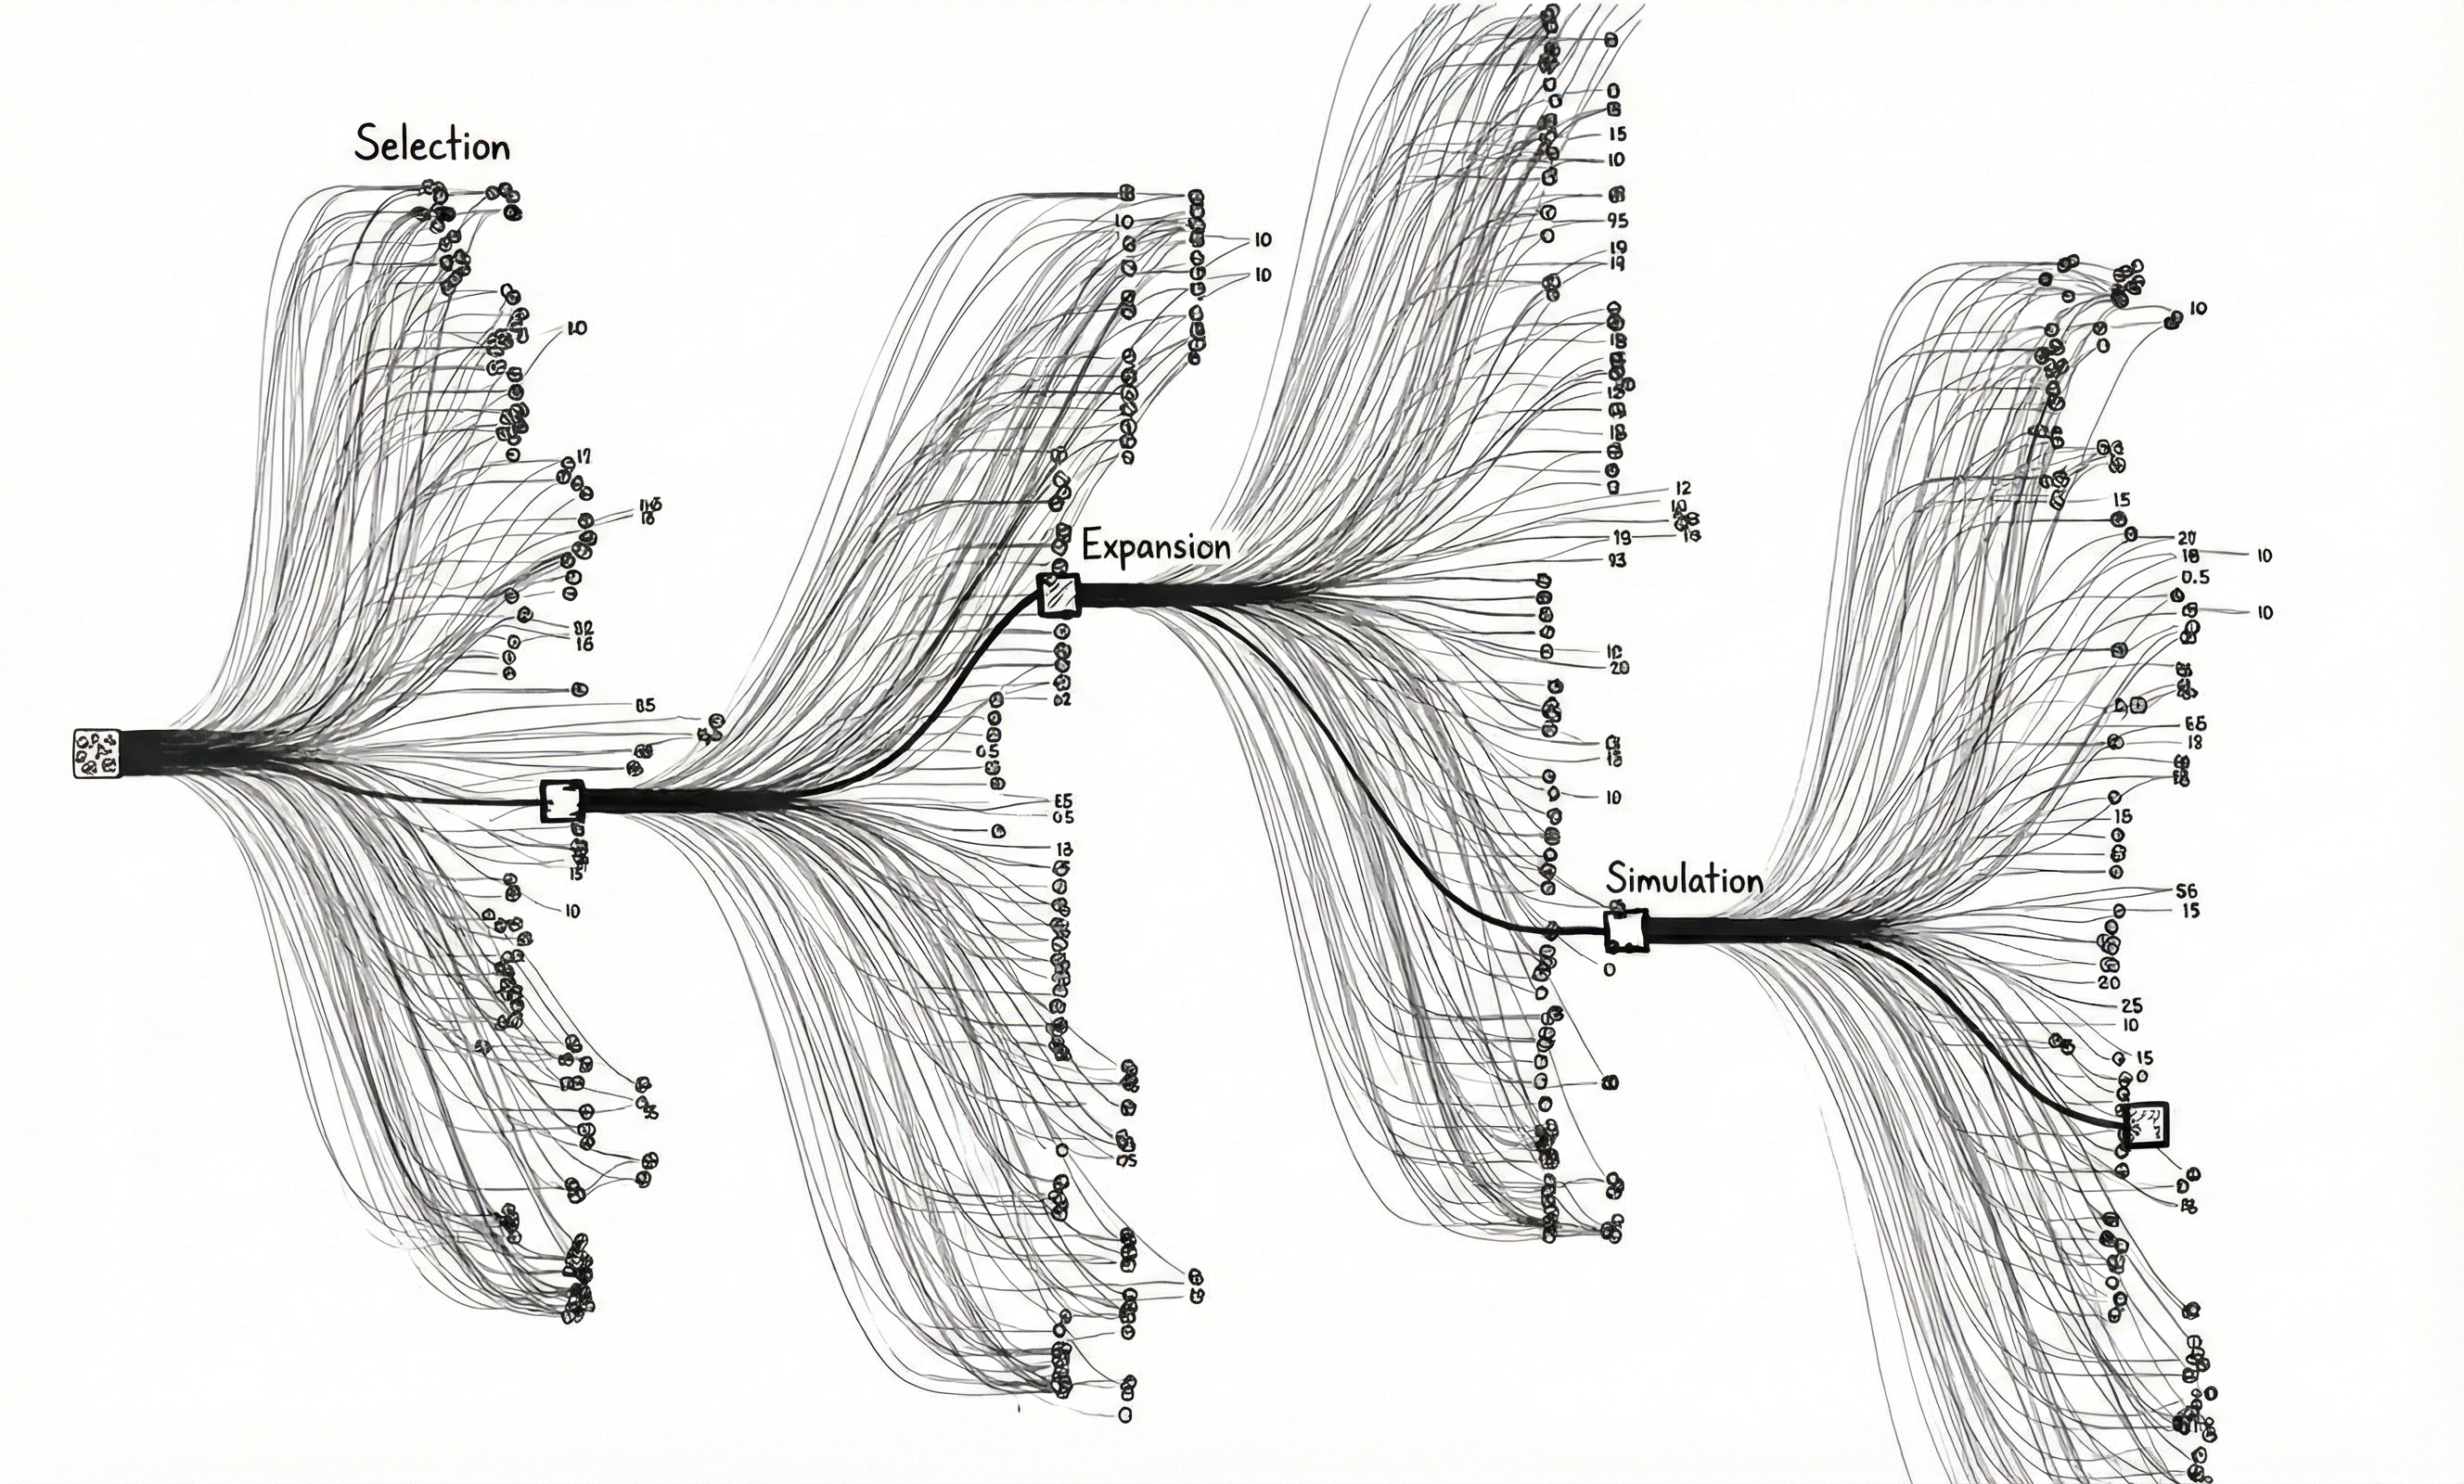
\includegraphics[width=\textwidth,height=0.5\textheight,keepaspectratio]{images/MCTS.png}
            \vspace{-0.5cm}
            \begin{itemize}
                \small
                \item 环境/状态:$T_n$
                \item 动作:策略头
                \item 奖励:价值头
            \end{itemize}
        \end{column}
        
        \begin{column}{0.85\textwidth}
            \centering
            \textbf{AlphaTensor架构}
            \vspace{0.3cm}
            \includegraphics[width=\textwidth,height=0.7\textheight,keepaspectratio]{images/jiagou.png}
        \end{column}
    \end{columns}
\end{frame}

\begin{frame}{网络架构与搜索算法}
    \begin{itemize}
        \item \textbf{MCTS}:用于规划下一步动作,平衡探索(Explore)与利用(Exploit)
        \item \textbf{Torso}:当前时间$T$,提取张量 $T \times T_n$ 的嵌入特征
        \item \textbf{Policy Head}:依次输出$k$个令牌,与$u \otimes v \otimes w$等价,每个token的维度为$d$,其中$k \times d = 3S$
        \item \textbf{Value Head}:预测奖励,即当前状态归零所需的最小步数
    \end{itemize}
    \vspace{-0.4cm}
    \begin{center}
        \includegraphics[width=0.8\textwidth,height=0.6\textheight,keepaspectratio]{images/network_architecture.png}
    \end{center}
\end{frame}

\begin{frame}{AlphaTensor架构细节1}
    \begin{center}
        \includegraphics[width=1.2\textwidth,height=0.40\textheight,keepaspectratio]{images/Torso diagram.png}
    \end{center}
    
    \begin{columns}[T]
        \begin{column}{0.6\textwidth}
            \begin{itemize}
                \small\small
                \item \textbf{Torso},输入历史张量$T \times S \times S \times S$,输出嵌入特征$3S^2 \times c$
                \item \textbf{Value Head},输入小向量$1 \times c$,输出小向量$1 \times q$
                \item \textbf{超参数},$c = 512, q = 128$
            \end{itemize}
        \end{column}
        \begin{column}{0.5\textwidth}
            \vspace{0.5cm}
            \includegraphics[width=1.0\textwidth,height=0.4\textheight,keepaspectratio]{images/value head diagram.png}
        \end{column}
    \end{columns}
\end{frame}

\begin{frame}{AlphaTensor架构细节2}
    \vspace{-0.3cm}
    \begin{columns}[T]
        \begin{column}{0.4\textwidth}
            \vspace{1.5cm}
            \begin{itemize}
                \small\small
                \item \textbf{Policy Head},输入零向量$1 \times d$与嵌入特征$3S^2 \times c$,输出令牌$1 \times d$,重复$k$次
                \item \textbf{超参数},$d=S , k=3 , c = 512$
            \end{itemize}
        \end{column}
        \begin{column}{0.6\textwidth}
            \includegraphics[width=0.9\textwidth,height=0.9\textheight,keepaspectratio]{images/policy head diagram.png}
        \end{column}
    \end{columns}
\end{frame}

% =======================================================
\section{实验结果}

\begin{frame}{理论突破:发现更优的秩}
    \begin{table}[h]
        \centering
        \caption{AlphaTensor 在不同矩阵尺寸下的发现}
        \begin{tabular}{c|c|c}
            \toprule
            矩阵尺寸 ($n,m,k$) & 现有最佳秩 (Human) & AlphaTensor \\
            \midrule
            $4, 4, 4$ & 49 (Strassen$^2$) & \textbf{47} \\
            $5, 5, 5$ & 98 & \textbf{96} \\
            $4, 5, 5$ & 80 & \textbf{76} \\
            \bottomrule
        \end{tabular}
    \end{table}
    \begin{itemize}
        \item AlphaTensor 在多种尺寸下发现了比人类已知算法更少的乘法次数。
        \item \textbf{注}:寻找矩阵最小的低秩分解,是np-hard问题。$3 \times 3$ 矩阵乘法已知的最小秩为23,但全局最优解仍然未知,本文也未攻克。
    \end{itemize}
\end{frame}

\begin{frame}{理论突破:不同矩阵乘法的最小秩}
    \begin{center}
        \includegraphics[width=\textwidth,height=0.85\textheight,keepaspectratio]{images/best_rank_known.png}
    \end{center}
\end{frame}

\begin{frame}{理论突破:4*4*4矩阵的低秩分解}
    \begin{columns}[T]
        \begin{column}{0.5\textwidth}
            \centering\vspace{1.5cm}
            \includegraphics[width=\textwidth,height=0.4\textheight,keepaspectratio]{images/444_up.png}
            \vspace{0.2cm}
            \includegraphics[width=0.55\textwidth,height=0.4\textheight,keepaspectratio]{images/444_down.png}
        \end{column}
        \begin{column}{0.5\textwidth}
            \centering
            \includegraphics[width=\textwidth,height=0.85\textheight,keepaspectratio]{images/444_new_find.png}
        \end{column}
    \end{columns}
\end{frame}

\begin{frame}{实际应用:硬件加速}
    AlphaTensor理论上减少了计算次数,并针对特定硬件(GPU V100, TPU v3)进行优化。
    
    \begin{exampleblock}{Runtime 优化}
        \begin{itemize}
            \item 理论上,在大尺寸矩阵 ($ > 8192$) 上,AlphaTensor 发现的算法在 GPU/TPU 上均有显著加速。
            \item 理论上,超越了标准的 cuBLAS 库性能。
        \end{itemize}
    \end{exampleblock}

    \begin{itemize}
        \item 理论上,在矩阵尺寸增大时,加速比显著提升。
        \item 理论上,证明了 AI 发现的算法具有更强的加速效果。
    \end{itemize}
\end{frame}

\begin{frame}{实际应用:加速效果}
    \begin{center}
        \includegraphics[width=\textwidth,height=0.85\textheight,keepaspectratio]{images/results.png}
    \end{center}
\end{frame}

\begin{frame}{消融实验}
    \framesubtitle{以 $4 \times 4 \times 4$ 矩阵为例}
    \begin{table}[h]
        \centering
        \small
        \begin{tabular}{l|c}
            \toprule
            \textbf{消融条件} & \textbf{发现的秩} \\
            \midrule
            Without \textit{synthetic demonstrations} & 64 \\
            Without \textit{selfplay} (supervised only) & 60 \\
            Without \textit{change of basis} & 58 \\
            Without \textit{signed permutations} & 53 \\
            Without retraining on best games 10\% of the time & 52 \\
            Without \textit{QR head} (using a \textit{categorical head}) & 52 \\
            \midrule
            \textbf{AlphaTensor (完整版)} & \textbf{49} \\
            \bottomrule
        \end{tabular}
    \end{table}
    
    \vspace{0.3cm}
    
    \begin{block}{结论}
        \small
        完整的AlphaTensor达到最优性能(Rank = 49)。移除任何组件都会导致性能下降,其中\textit{synthetic demonstrations}(合成演示)的影响最大。
    \end{block}
\end{frame}

\begin{frame}{复现结果:模型训练}
    \begin{center}
        \begin{columns}[T]
            \begin{column}{0.45\textwidth}
                \begin{itemize}
                    \item 复现工作主要有两部分
                \end{itemize}
                \begin{enumerate}
                    \item 复现强化学习模型训练,使用OpenTensor开源代码
                    \item 复现最小的矩阵乘法次数的加速效果,使用AlphaTensor开源代码
                \end{enumerate}
            \end{column}
            \begin{column}{0.5\textwidth}
                \includegraphics[width=1.0\textwidth,keepaspectratio]{images/nvidia-smi.png}
            \end{column}
        \end{columns}
        
        \vspace{0.2cm}
        \includegraphics[width=1.0\textwidth,keepaspectratio]{images/RL_training.png}
    \end{center}
\end{frame}

\begin{frame}{复现结果:加速效果}
    \vspace{-0.3cm}
    \begin{columns}[T]
        \begin{column}{0.48\textwidth}
            \centering
            \includegraphics[width=\textwidth,keepaspectratio]{images/result_left.png}
        \end{column}
        \begin{column}{0.5\textwidth}
            \centering
            \includegraphics[width=\textwidth,keepaspectratio]{images/result_middle.png}
        \end{column}
    \end{columns}
\end{frame}

\begin{frame}{复现结果:对照}
    \begin{table}[h]
        \centering
        \small
        \begin{tabular}{c|c|c|c|c}
            \toprule
            \multirow{2}{*}{\textbf{矩阵尺寸}} & \multicolumn{2}{c|}{\textbf{Strassen$^2$}} & \multicolumn{2}{c}{\textbf{AlphaTensor}} \\
            \cmidrule(lr){2-3} \cmidrule(lr){4-5}
            & \textbf{复现} & \textbf{原文} & \textbf{复现} & \textbf{原文} \\
            \midrule
            $8192 $ & 5.35 & 4.3 & 8.55 & 8.5 \\
            $10240 $ & 15.98 & 6.8 & 19.11 & 10.7 \\
            $12288 $ & 14.53 & 10.1 & 17.09 & 13.3 \\
            $14336 $ & 18.53 & 16.1 & 20.82 & 19.6 \\
            $16384 $ & 17.61 & 13.8 & 19.60 & 16.6 \\
            $18432 $ & 19.28 & 15.3 & 20.99 & 17.9 \\
            $20480 $ & 24.04 & 21.3 & 25.84 & 23.9 \\
            \bottomrule
        \end{tabular}
        \caption{不同算法相对于 jnp.dot 的加速比(单位:\%)}
    \end{table}
    \begin{itemize}
        \item 相对地,AlphaTensor比标准库与Strassen$^2$都快
        \item 绝对地,AlphaTensor运算8192矩阵乘法的时间近1分钟,运算20480矩阵乘法的时间近8分钟,远远慢于标准矩阵乘法。
    \end{itemize}
\end{frame}

% =======================================================
\section{总结展望}

\begin{frame}{文章局限:工业实践角度}
    \textbf{\textcolor{blue}{硬件指令集的冲突}}
    \begin{itemize}
        \item \textbf{现代GPU}均以\textcolor{blue}{Tensor Cores}为计算核心,这些硬件单元在物理电路层面,针对标准的$O(N^3)$算法逻辑进行高度优化。
        \item \textbf{AlphaTensor}减少了乘法操作,但将内存开销由$O(2N)$\textbf{暴增}到$O(N^{2})$,得不偿失。
    \end{itemize}
    
    \textbf{\textcolor{blue}{数值稳定性}}
    \begin{itemize}
        \item \textbf{标准库}倾向于选择\textbf{最稳定}的算法而非理论上最快的。
        \item \textbf{AlphaTensor}通过复杂的加减法组合减少乘法,在浮点运算中容易引入\textcolor{red}{精度损失},数值稳定性差。
    \end{itemize}

    \begin{block}{结论}
        \begin{itemize}
            \item Strassen的年代,内存访问很慢,所以才开辟用数学优化矩阵乘法的道路。
            \item 现在内存访问快,数据处理量大,优化矩阵乘法要靠系统层面整体的优化,不能只靠数学层面的取巧。
        \end{itemize}
    \end{block}

\end{frame}


\begin{frame}{文章局限:学术引用角度}

    \begin{itemize}
        \item 优化矩阵计算领域,AlphaTensor是久违的重大突破
        \item 强化学习领域,论文引用数逐年减少,学术热度下降。引用数主要出自综述
    \end{itemize}
    
    \vspace{0.5cm}
    
    \begin{columns}[T]
        \begin{column}{0.3\textwidth}
            \centering
            \includegraphics[width=\textwidth,height=0.45\textheight,keepaspectratio]{images/alphatensor_citation.png}
            \tiny AlphaTensor
        \end{column}
        
        \begin{column}{0.3\textwidth}
            \centering
            \includegraphics[width=\textwidth,height=0.45\textheight,keepaspectratio]{images/alphatensor_connected.png}
        \end{column}
        
        \begin{column}{0.3\textwidth}
            \centering
            \includegraphics[width=\textwidth,height=0.45\textheight,keepaspectratio]{images/alphafold_citation.png}
            \tiny AlphaFold
        \end{column}
        
        \begin{column}{0.3\textwidth}
            \centering
            \includegraphics[width=\textwidth,height=0.45\textheight,keepaspectratio]{images/alphafold_connected.png}
        \end{column}
    \end{columns}
\end{frame}

\begin{frame}{文章贡献}
    \begin{itemize}        
        \item \textbf{矩阵加速}
        \begin{itemize}
            \item  AlphaTensor 将大矩阵乘法次数的下界从$O(N^{2.807})$降低到了$O(N^{2.777})$。
        \end{itemize}

        \item \textbf{AI for Science}
        \begin{itemize}
            \item 继 AlphaGo (围棋)、AlphaFold (蛋白质) 之后,DeepMind 在基础数学/理论计算机领域的突破。是强化学习的又一次成功应用。
        \end{itemize}

        \item \textbf{未来展望}
        \begin{itemize}
            \item 优化其他经典算法/理论计算机科学方法的算法流程?
            \item 解决其他np-hard问题?
            \item 把强化学习这种思想,全面引入传统理工科?
        \end{itemize}
    \end{itemize}
\end{frame}

\begin{frame}[allowframebreaks]{参考资料}
    \nocite{*}
    \bibliography{refe}
    \tiny\bibliographystyle{alpha}
\end{frame}

\begin{frame}{人员分工}
    \small
    \setlength{\tabcolsep}{12pt}
    \renewcommand{\arraystretch}{1.5}
    \begin{flushleft}
        \begin{tabular}{c|c}
            李致远 & 选题,复现,演讲 \\
            冯文喆 & 背景调研部分 \\
            魏睿 & 核心原理部分 \\
            宋泽顷 & 实验结果与总结展望部分 \\
            周启民 & 幻灯片 \\
        \end{tabular}
    \end{flushleft}
    
    \vspace{0.3cm}
    
    \begin{flushleft}
        \small
        \textbf{项目地址}:
        \begin{itemize}
            \item \url{https://gitee.com/lychee-garden/pre_alphatensor.git}
            \item \url{https://gitee.com/lychee-garden/pre_opentensor.git}
            \item \url{https://gitee.com/lychee-garden/alphatensor_slides.git}
        \end{itemize}
    \end{flushleft}
\end{frame}

\begin{frame}
	\begin{center}
		{\Huge\calligra Thanks!}
	\end{center}
\end{frame}

\end{document}